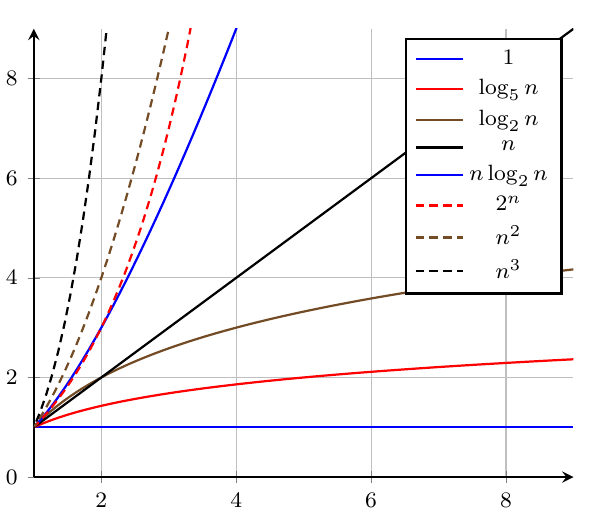
\begin{tikzpicture}
    \begin{axis}
      [
      axis lines = left,
      xmin=1, xmax=9, ymin=0, ymax=9,
      domain=0:9, samples=100, no markers, thick, grid=both,
      xlabel = {Increasing \(n\)}, ylabel = {\(f(n)\)},
      label style = {overlay},       % Has he same effect as
      ticklabel style = {overlay},   % trim axis [left|right]
      legend entries = {
        $1$,
        $\log_{5}n$,
        $\log_{2}n$,
        $n$,
        $n\log_{2}n$,
        $2^{n}$,
        $n^{2}$,
        $n^{3}$,
      },
      every axis/.style = {font=\footnotesize},
      label style = {font=\normalsize},
      ]
      \addplot+ {1};
      \addplot+ {1 + ln(x)/ln(5)};
      \addplot+ {1 + ln(x)/ln(2)};
      \addplot+ {x};
      \addplot+ {1 + x*ln(x)/ln(2)};
      \addplot+ {2^x-1};
      \addplot+ {x^2};
      \addplot+ {x^3};
    \end{axis}
  \end{tikzpicture}